% Options for packages loaded elsewhere
\PassOptionsToPackage{unicode}{hyperref}
\PassOptionsToPackage{hyphens}{url}
%
\documentclass[
]{article}
\usepackage{lmodern}
\usepackage{amsmath}
\usepackage{ifxetex,ifluatex}
\ifnum 0\ifxetex 1\fi\ifluatex 1\fi=0 % if pdftex
  \usepackage[T1]{fontenc}
  \usepackage[utf8]{inputenc}
  \usepackage{textcomp} % provide euro and other symbols
  \usepackage{amssymb}
\else % if luatex or xetex
  \usepackage{unicode-math}
  \defaultfontfeatures{Scale=MatchLowercase}
  \defaultfontfeatures[\rmfamily]{Ligatures=TeX,Scale=1}
\fi
% Use upquote if available, for straight quotes in verbatim environments
\IfFileExists{upquote.sty}{\usepackage{upquote}}{}
\IfFileExists{microtype.sty}{% use microtype if available
  \usepackage[]{microtype}
  \UseMicrotypeSet[protrusion]{basicmath} % disable protrusion for tt fonts
}{}
\makeatletter
\@ifundefined{KOMAClassName}{% if non-KOMA class
  \IfFileExists{parskip.sty}{%
    \usepackage{parskip}
  }{% else
    \setlength{\parindent}{0pt}
    \setlength{\parskip}{6pt plus 2pt minus 1pt}}
}{% if KOMA class
  \KOMAoptions{parskip=half}}
\makeatother
\usepackage{xcolor}
\IfFileExists{xurl.sty}{\usepackage{xurl}}{} % add URL line breaks if available
\IfFileExists{bookmark.sty}{\usepackage{bookmark}}{\usepackage{hyperref}}
\hypersetup{
  hidelinks,
  pdfcreator={LaTeX via pandoc}}
\urlstyle{same} % disable monospaced font for URLs
\usepackage[margin=1in]{geometry}
\usepackage{longtable,booktabs}
\usepackage{calc} % for calculating minipage widths
% Correct order of tables after \paragraph or \subparagraph
\usepackage{etoolbox}
\makeatletter
\patchcmd\longtable{\par}{\if@noskipsec\mbox{}\fi\par}{}{}
\makeatother
% Allow footnotes in longtable head/foot
\IfFileExists{footnotehyper.sty}{\usepackage{footnotehyper}}{\usepackage{footnote}}
\makesavenoteenv{longtable}
\usepackage{graphicx}
\makeatletter
\def\maxwidth{\ifdim\Gin@nat@width>\linewidth\linewidth\else\Gin@nat@width\fi}
\def\maxheight{\ifdim\Gin@nat@height>\textheight\textheight\else\Gin@nat@height\fi}
\makeatother
% Scale images if necessary, so that they will not overflow the page
% margins by default, and it is still possible to overwrite the defaults
% using explicit options in \includegraphics[width, height, ...]{}
\setkeys{Gin}{width=\maxwidth,height=\maxheight,keepaspectratio}
% Set default figure placement to htbp
\makeatletter
\def\fps@figure{htbp}
\makeatother
\setlength{\emergencystretch}{3em} % prevent overfull lines
\providecommand{\tightlist}{%
  \setlength{\itemsep}{0pt}\setlength{\parskip}{0pt}}
\setcounter{secnumdepth}{-\maxdimen} % remove section numbering
\usepackage{booktabs}
\usepackage{longtable}
\usepackage{array}
\usepackage{multirow}
\usepackage{wrapfig}
\usepackage{float}
\usepackage{colortbl}
\usepackage{pdflscape}
\usepackage{tabu}
\usepackage{threeparttable}
\usepackage{threeparttablex}
\usepackage[normalem]{ulem}
\usepackage{makecell}
\usepackage{xcolor}
\ifluatex
  \usepackage{selnolig}  % disable illegal ligatures
\fi

\author{}
\date{\vspace{-2.5em}}

\begin{document}

\hypertarget{section}{%
\subsection{2002-2009}\label{section}}

\begin{table}[!ht]

\caption{\label{tab:unnamed-chunk-2}2002-2009}
\centering
\fontsize{10}{12}\selectfont
\begin{tabular}[t]{lccccc}
\toprule
 & ICEWS & GED & CINEP & \makecell[c]{ICEWS\\Underreporing} & \makecell[c]{GED\\Underreporting}\\
\midrule
 & \bgroup\fontsize{10}{12}\selectfont  -5.662\egroup{} & \bgroup\fontsize{10}{12}\selectfont  -7.239\egroup{} & \bgroup\fontsize{10}{12}\selectfont  -8.324\egroup{} & \bgroup\fontsize{10}{12}\selectfont  -4.223\egroup{} & \bgroup\fontsize{10}{12}\selectfont  -3.336\egroup{}\\

\multirow{-2}{*}{\raggedright\arraybackslash Intercept} & \bgroup\fontsize{8}{10}\selectfont [ -7.809,   -3.512]\egroup{} & \bgroup\fontsize{8}{10}\selectfont [-11.281,   -3.917]\egroup{} & \bgroup\fontsize{8}{10}\selectfont [-13.707,   -4.154]\egroup{} & \bgroup\fontsize{8}{10}\selectfont [ -8.652,   -0.771]\egroup{} & \bgroup\fontsize{8}{10}\selectfont [ -6.367,   -0.588]\egroup{}\\

 & \bgroup\fontsize{10}{12}\selectfont   0.211\egroup{} & \bgroup\fontsize{10}{12}\selectfont   0.408\egroup{} & \bgroup\fontsize{10}{12}\selectfont   0.595\egroup{} & \bgroup\fontsize{10}{12}\selectfont   0.264\egroup{} & \bgroup\fontsize{10}{12}\selectfont   0.156\egroup{}\\

\multirow{-2}{*}{\raggedright\arraybackslash Dist. Bogota, km (log)} & \bgroup\fontsize{8}{10}\selectfont [ -0.111,    0.518]\egroup{} & \bgroup\fontsize{8}{10}\selectfont [ -0.081,    0.980]\egroup{} & \bgroup\fontsize{8}{10}\selectfont [ -0.040,    1.388]\egroup{} & \bgroup\fontsize{8}{10}\selectfont [ -0.266,    0.935]\egroup{} & \bgroup\fontsize{8}{10}\selectfont [ -0.261,    0.610]\egroup{}\\

 & \bgroup\fontsize{10}{12}\selectfont   0.355\egroup{} & \bgroup\fontsize{10}{12}\selectfont   0.368\egroup{} & \bgroup\fontsize{10}{12}\selectfont   0.376\egroup{} & \bgroup\fontsize{10}{12}\selectfont   0.140\egroup{} & \bgroup\fontsize{10}{12}\selectfont   0.110\egroup{}\\

\multirow{-2}{*}{\raggedright\arraybackslash Population (log)} & \bgroup\fontsize{8}{10}\selectfont [  0.260,    0.454]\egroup{} & \bgroup\fontsize{8}{10}\selectfont [  0.267,    0.473]\egroup{} & \bgroup\fontsize{8}{10}\selectfont [  0.275,    0.479]\egroup{} & \bgroup\fontsize{8}{10}\selectfont [  0.039,    0.241]\egroup{} & \bgroup\fontsize{8}{10}\selectfont [  0.008,    0.208]\egroup{}\\

 & \bgroup\fontsize{10}{12}\selectfont   0.006\egroup{} & \bgroup\fontsize{10}{12}\selectfont   0.014\egroup{} & \bgroup\fontsize{10}{12}\selectfont   0.018\egroup{} & \bgroup\fontsize{10}{12}\selectfont   0.010\egroup{} & \bgroup\fontsize{10}{12}\selectfont   0.007\egroup{}\\

\multirow{-2}{*}{\raggedright\arraybackslash TRI} & \bgroup\fontsize{8}{10}\selectfont [  0.000,    0.013]\egroup{} & \bgroup\fontsize{8}{10}\selectfont [  0.007,    0.020]\egroup{} & \bgroup\fontsize{8}{10}\selectfont [  0.011,    0.024]\egroup{} & \bgroup\fontsize{8}{10}\selectfont [  0.003,    0.016]\egroup{} & \bgroup\fontsize{8}{10}\selectfont [  0.001,    0.013]\egroup{}\\
\cline{1-6}

 & \bgroup\fontsize{10}{12}\selectfont   5.675\egroup{} & \bgroup\fontsize{10}{12}\selectfont   0.994\egroup{} & \bgroup\fontsize{10}{12}\selectfont   1.258\egroup{} & \bgroup\fontsize{10}{12}\selectfont   1.542\egroup{} & \bgroup\fontsize{10}{12}\selectfont   1.943\egroup{}\\

\multirow{-2}{*}{\raggedright\arraybackslash Kappa} & \bgroup\fontsize{8}{10}\selectfont [  0.832,   24.057]\egroup{} & \bgroup\fontsize{8}{10}\selectfont [  0.387,    1.898]\egroup{} & \bgroup\fontsize{8}{10}\selectfont [  0.576,    2.301]\egroup{} & \bgroup\fontsize{8}{10}\selectfont [  0.617,    3.035]\egroup{} & \bgroup\fontsize{8}{10}\selectfont [  0.572,    4.727]\egroup{}\\

 & \bgroup\fontsize{10}{12}\selectfont   1.265\egroup{} & \bgroup\fontsize{10}{12}\selectfont   0.792\egroup{} & \bgroup\fontsize{10}{12}\selectfont   2.021\egroup{} & \bgroup\fontsize{10}{12}\selectfont   1.039\egroup{} & \bgroup\fontsize{10}{12}\selectfont   0.621\egroup{}\\

\multirow{-2}{*}{\raggedright\arraybackslash Sigma} & \bgroup\fontsize{8}{10}\selectfont [  0.064,    8.324]\egroup{} & \bgroup\fontsize{8}{10}\selectfont [  0.302,    1.565]\egroup{} & \bgroup\fontsize{8}{10}\selectfont [  0.928,    3.591]\egroup{} & \bgroup\fontsize{8}{10}\selectfont [  0.481,    1.861]\egroup{} & \bgroup\fontsize{8}{10}\selectfont [  0.196,    1.402]\egroup{}\\

 & \bgroup\fontsize{10}{12}\selectfont  55.046\egroup{} & \bgroup\fontsize{10}{12}\selectfont 315.849\egroup{} & \bgroup\fontsize{10}{12}\selectfont 249.654\egroup{} & \bgroup\fontsize{10}{12}\selectfont 203.601\egroup{} & \bgroup\fontsize{10}{12}\selectfont 161.467\egroup{}\\

\multirow{-2}{*}{\raggedright\arraybackslash Range} & \bgroup\fontsize{8}{10}\selectfont [  3.375,  156.224]\egroup{} & \bgroup\fontsize{8}{10}\selectfont [123.612,  605.266]\egroup{} & \bgroup\fontsize{8}{10}\selectfont [108.404,  436.257]\egroup{} & \bgroup\fontsize{8}{10}\selectfont [ 76.615,  381.758]\egroup{} & \bgroup\fontsize{8}{10}\selectfont [ 39.859,  348.192]\egroup{}\\
\cline{1-6}

LogLik & \bgroup\fontsize{10}{12}\selectfont -465.646\egroup{} & \bgroup\fontsize{10}{12}\selectfont -452.414\egroup{} & \bgroup\fontsize{10}{12}\selectfont -527.630\egroup{} & \bgroup\fontsize{10}{12}\selectfont -492.083\egroup{} & \bgroup\fontsize{10}{12}\selectfont -475.855\egroup{}\\

N & \bgroup\fontsize{10}{12}\selectfont 1116\egroup{} & \bgroup\fontsize{10}{12}\selectfont 1116\egroup{} & \bgroup\fontsize{10}{12}\selectfont 1116\egroup{} & \bgroup\fontsize{10}{12}\selectfont 1116\egroup{} & \bgroup\fontsize{10}{12}\selectfont 1116\egroup{}\\
\bottomrule
\end{tabular}
\end{table}

\hypertarget{section-1}{%
\subsection{2002-2004}\label{section-1}}

\begin{table}[!ht]

\caption{\label{tab:unnamed-chunk-3}2002-2004}
\centering
\fontsize{10}{12}\selectfont
\begin{tabular}[t]{lccccc}
\toprule
 & ICEWS & GED & CINEP & \makecell[c]{ICEWS\\Underreporing} & \makecell[c]{GED\\Underreporting}\\
\midrule
 & \bgroup\fontsize{10}{12}\selectfont  -3.820\egroup{} & \bgroup\fontsize{10}{12}\selectfont  -5.566\egroup{} & \bgroup\fontsize{10}{12}\selectfont  -7.125\egroup{} & \bgroup\fontsize{10}{12}\selectfont  -5.881\egroup{} & \bgroup\fontsize{10}{12}\selectfont  -3.897\egroup{}\\

\multirow{-2}{*}{\raggedright\arraybackslash Intercept} & \bgroup\fontsize{8}{10}\selectfont [ -6.177,   -0.888]\egroup{} & \bgroup\fontsize{8}{10}\selectfont [ -9.154,   -2.564]\egroup{} & \bgroup\fontsize{8}{10}\selectfont [-11.724,   -3.420]\egroup{} & \bgroup\fontsize{8}{10}\selectfont [-10.661,   -2.154]\egroup{} & \bgroup\fontsize{8}{10}\selectfont [ -7.183,   -1.152]\egroup{}\\

 & \bgroup\fontsize{10}{12}\selectfont  -0.018\egroup{} & \bgroup\fontsize{10}{12}\selectfont   0.161\egroup{} & \bgroup\fontsize{10}{12}\selectfont   0.417\egroup{} & \bgroup\fontsize{10}{12}\selectfont   0.392\egroup{} & \bgroup\fontsize{10}{12}\selectfont   0.197\egroup{}\\

\multirow{-2}{*}{\raggedright\arraybackslash Dist. Bogota, km (log)} & \bgroup\fontsize{8}{10}\selectfont [ -0.453,    0.317]\egroup{} & \bgroup\fontsize{8}{10}\selectfont [ -0.262,    0.640]\egroup{} & \bgroup\fontsize{8}{10}\selectfont [ -0.148,    1.097]\egroup{} & \bgroup\fontsize{8}{10}\selectfont [ -0.177,    1.102]\egroup{} & \bgroup\fontsize{8}{10}\selectfont [ -0.218,    0.688]\egroup{}\\

 & \bgroup\fontsize{10}{12}\selectfont   0.278\egroup{} & \bgroup\fontsize{10}{12}\selectfont   0.339\egroup{} & \bgroup\fontsize{10}{12}\selectfont   0.355\egroup{} & \bgroup\fontsize{10}{12}\selectfont   0.227\egroup{} & \bgroup\fontsize{10}{12}\selectfont   0.137\egroup{}\\

\multirow{-2}{*}{\raggedright\arraybackslash Population (log)} & \bgroup\fontsize{8}{10}\selectfont [  0.177,    0.382]\egroup{} & \bgroup\fontsize{8}{10}\selectfont [  0.237,    0.445]\egroup{} & \bgroup\fontsize{8}{10}\selectfont [  0.254,    0.458]\egroup{} & \bgroup\fontsize{8}{10}\selectfont [  0.126,    0.328]\egroup{} & \bgroup\fontsize{8}{10}\selectfont [  0.036,    0.237]\egroup{}\\

 & \bgroup\fontsize{10}{12}\selectfont   0.004\egroup{} & \bgroup\fontsize{10}{12}\selectfont   0.007\egroup{} & \bgroup\fontsize{10}{12}\selectfont   0.016\egroup{} & \bgroup\fontsize{10}{12}\selectfont   0.011\egroup{} & \bgroup\fontsize{10}{12}\selectfont   0.009\egroup{}\\

\multirow{-2}{*}{\raggedright\arraybackslash TRI} & \bgroup\fontsize{8}{10}\selectfont [ -0.002,    0.011]\egroup{} & \bgroup\fontsize{8}{10}\selectfont [  0.001,    0.014]\egroup{} & \bgroup\fontsize{8}{10}\selectfont [  0.010,    0.023]\egroup{} & \bgroup\fontsize{8}{10}\selectfont [  0.005,    0.018]\egroup{} & \bgroup\fontsize{8}{10}\selectfont [  0.003,    0.015]\egroup{}\\
\cline{1-6}

 & \bgroup\fontsize{10}{12}\selectfont   1.189\egroup{} & \bgroup\fontsize{10}{12}\selectfont   0.886\egroup{} & \bgroup\fontsize{10}{12}\selectfont   1.293\egroup{} & \bgroup\fontsize{10}{12}\selectfont   1.186\egroup{} & \bgroup\fontsize{10}{12}\selectfont   1.707\egroup{}\\

\multirow{-2}{*}{\raggedright\arraybackslash Kappa} & \bgroup\fontsize{8}{10}\selectfont [  0.217,    3.822]\egroup{} & \bgroup\fontsize{8}{10}\selectfont [  0.269,    1.924]\egroup{} & \bgroup\fontsize{8}{10}\selectfont [  0.562,    2.394]\egroup{} & \bgroup\fontsize{8}{10}\selectfont [  0.488,    2.323]\egroup{} & \bgroup\fontsize{8}{10}\selectfont [  0.513,    4.015]\egroup{}\\

 & \bgroup\fontsize{10}{12}\selectfont   0.284\egroup{} & \bgroup\fontsize{10}{12}\selectfont   0.489\egroup{} & \bgroup\fontsize{10}{12}\selectfont   1.395\egroup{} & \bgroup\fontsize{10}{12}\selectfont   1.094\egroup{} & \bgroup\fontsize{10}{12}\selectfont   0.579\egroup{}\\

\multirow{-2}{*}{\raggedright\arraybackslash Sigma} & \bgroup\fontsize{8}{10}\selectfont [  0.059,    0.692]\egroup{} & \bgroup\fontsize{8}{10}\selectfont [  0.142,    1.101]\egroup{} & \bgroup\fontsize{8}{10}\selectfont [  0.622,    2.544]\egroup{} & \bgroup\fontsize{8}{10}\selectfont [  0.454,    2.084]\egroup{} & \bgroup\fontsize{8}{10}\selectfont [  0.200,    1.214]\egroup{}\\

 & \bgroup\fontsize{10}{12}\selectfont 263.306\egroup{} & \bgroup\fontsize{10}{12}\selectfont 354.148\egroup{} & \bgroup\fontsize{10}{12}\selectfont 242.868\egroup{} & \bgroup\fontsize{10}{12}\selectfont 264.714\egroup{} & \bgroup\fontsize{10}{12}\selectfont 183.858\egroup{}\\

\multirow{-2}{*}{\raggedright\arraybackslash Range} & \bgroup\fontsize{8}{10}\selectfont [ 33.073,  690.542]\egroup{} & \bgroup\fontsize{8}{10}\selectfont [106.760,  765.170]\egroup{} & \bgroup\fontsize{8}{10}\selectfont [102.152,  437.736]\egroup{} & \bgroup\fontsize{8}{10}\selectfont [101.292,  488.888]\egroup{} & \bgroup\fontsize{8}{10}\selectfont [ 48.321,  393.481]\egroup{}\\
\cline{1-6}

LogLik & \bgroup\fontsize{10}{12}\selectfont -369.389\egroup{} & \bgroup\fontsize{10}{12}\selectfont -392.993\egroup{} & \bgroup\fontsize{10}{12}\selectfont -504.872\egroup{} & \bgroup\fontsize{10}{12}\selectfont -477.819\egroup{} & \bgroup\fontsize{10}{12}\selectfont -456.209\egroup{}\\

N & \bgroup\fontsize{10}{12}\selectfont 1116\egroup{} & \bgroup\fontsize{10}{12}\selectfont 1116\egroup{} & \bgroup\fontsize{10}{12}\selectfont 1116\egroup{} & \bgroup\fontsize{10}{12}\selectfont 1116\egroup{} & \bgroup\fontsize{10}{12}\selectfont 1116\egroup{}\\
\bottomrule
\end{tabular}
\end{table}

\pagebreak

\hypertarget{section-2}{%
\subsection{2005-2007}\label{section-2}}

\begin{table}[!ht]

\caption{\label{tab:unnamed-chunk-4}2005-2007}
\centering
\fontsize{10}{12}\selectfont
\begin{tabular}[t]{lccccc}
\toprule
 & ICEWS & GED & CINEP & \makecell[c]{ICEWS\\Underreporing} & \makecell[c]{GED\\Underreporting}\\
\midrule
 & \bgroup\fontsize{10}{12}\selectfont  -8.326\egroup{} & \bgroup\fontsize{10}{12}\selectfont  -9.877\egroup{} & \bgroup\fontsize{10}{12}\selectfont  -5.214\egroup{} & \bgroup\fontsize{10}{12}\selectfont  -3.228\egroup{} & \bgroup\fontsize{10}{12}\selectfont  -3.877\egroup{}\\

\multirow{-2}{*}{\raggedright\arraybackslash Intercept} & \bgroup\fontsize{8}{10}\selectfont [-11.461,   -5.813]\egroup{} & \bgroup\fontsize{8}{10}\selectfont [-23.989,    5.736]\egroup{} & \bgroup\fontsize{8}{10}\selectfont [-11.642,    0.316]\egroup{} & \bgroup\fontsize{8}{10}\selectfont [ -8.950,    2.097]\egroup{} & \bgroup\fontsize{8}{10}\selectfont [ -9.494,    1.561]\egroup{}\\

 & \bgroup\fontsize{10}{12}\selectfont   0.495\egroup{} & \bgroup\fontsize{10}{12}\selectfont   0.497\egroup{} & \bgroup\fontsize{10}{12}\selectfont   0.045\egroup{} & \bgroup\fontsize{10}{12}\selectfont  -0.082\egroup{} & \bgroup\fontsize{10}{12}\selectfont   0.017\egroup{}\\

\multirow{-2}{*}{\raggedright\arraybackslash Dist. Bogota, km (log)} & \bgroup\fontsize{8}{10}\selectfont [  0.131,    0.934]\egroup{} & \bgroup\fontsize{8}{10}\selectfont [ -0.232,    1.454]\egroup{} & \bgroup\fontsize{8}{10}\selectfont [ -0.883,    1.032]\egroup{} & \bgroup\fontsize{8}{10}\selectfont [ -0.978,    0.803]\egroup{} & \bgroup\fontsize{8}{10}\selectfont [ -0.900,    0.882]\egroup{}\\

 & \bgroup\fontsize{10}{12}\selectfont   0.409\egroup{} & \bgroup\fontsize{10}{12}\selectfont   0.420\egroup{} & \bgroup\fontsize{10}{12}\selectfont   0.300\egroup{} & \bgroup\fontsize{10}{12}\selectfont   0.163\egroup{} & \bgroup\fontsize{10}{12}\selectfont   0.184\egroup{}\\

\multirow{-2}{*}{\raggedright\arraybackslash Population (log)} & \bgroup\fontsize{8}{10}\selectfont [  0.295,    0.530]\egroup{} & \bgroup\fontsize{8}{10}\selectfont [  0.279,    0.570]\egroup{} & \bgroup\fontsize{8}{10}\selectfont [  0.162,    0.438]\egroup{} & \bgroup\fontsize{8}{10}\selectfont [  0.011,    0.310]\egroup{} & \bgroup\fontsize{8}{10}\selectfont [  0.033,    0.330]\egroup{}\\

 & \bgroup\fontsize{10}{12}\selectfont   0.005\egroup{} & \bgroup\fontsize{10}{12}\selectfont   0.019\egroup{} & \bgroup\fontsize{10}{12}\selectfont   0.007\egroup{} & \bgroup\fontsize{10}{12}\selectfont   0.004\egroup{} & \bgroup\fontsize{10}{12}\selectfont   0.002\egroup{}\\

\multirow{-2}{*}{\raggedright\arraybackslash TRI} & \bgroup\fontsize{8}{10}\selectfont [ -0.002,    0.014]\egroup{} & \bgroup\fontsize{8}{10}\selectfont [  0.009,    0.030]\egroup{} & \bgroup\fontsize{8}{10}\selectfont [ -0.002,    0.016]\egroup{} & \bgroup\fontsize{8}{10}\selectfont [ -0.005,    0.014]\egroup{} & \bgroup\fontsize{8}{10}\selectfont [ -0.007,    0.011]\egroup{}\\
\cline{1-6}

 & \bgroup\fontsize{10}{12}\selectfont   5.112\egroup{} & \bgroup\fontsize{10}{12}\selectfont   0.446\egroup{} & \bgroup\fontsize{10}{12}\selectfont   2.829\egroup{} & \bgroup\fontsize{10}{12}\selectfont   3.465\egroup{} & \bgroup\fontsize{10}{12}\selectfont   4.124\egroup{}\\

\multirow{-2}{*}{\raggedright\arraybackslash Kappa} & \bgroup\fontsize{8}{10}\selectfont [  0.800,   15.876]\egroup{} & \bgroup\fontsize{8}{10}\selectfont [  0.107,    0.955]\egroup{} & \bgroup\fontsize{8}{10}\selectfont [  1.236,    5.809]\egroup{} & \bgroup\fontsize{8}{10}\selectfont [  1.122,    9.154]\egroup{} & \bgroup\fontsize{8}{10}\selectfont [  1.371,   11.183]\egroup{}\\

 & \bgroup\fontsize{10}{12}\selectfont   1.334\egroup{} & \bgroup\fontsize{10}{12}\selectfont   1.679\egroup{} & \bgroup\fontsize{10}{12}\selectfont   4.141\egroup{} & \bgroup\fontsize{10}{12}\selectfont   4.547\egroup{} & \bgroup\fontsize{10}{12}\selectfont   5.764\egroup{}\\

\multirow{-2}{*}{\raggedright\arraybackslash Sigma} & \bgroup\fontsize{8}{10}\selectfont [  0.089,    4.628]\egroup{} & \bgroup\fontsize{8}{10}\selectfont [  0.182,    6.215]\egroup{} & \bgroup\fontsize{8}{10}\selectfont [  1.829,    8.377]\egroup{} & \bgroup\fontsize{8}{10}\selectfont [  0.766,   16.012]\egroup{} & \bgroup\fontsize{8}{10}\selectfont [  1.211,   19.988]\egroup{}\\

 & \bgroup\fontsize{10}{12}\selectfont  61.258\egroup{} & \bgroup\fontsize{10}{12}\selectfont 703.923\egroup{} & \bgroup\fontsize{10}{12}\selectfont 110.986\egroup{} & \bgroup\fontsize{10}{12}\selectfont  90.525\egroup{} & \bgroup\fontsize{10}{12}\selectfont  76.053\egroup{}\\

\multirow{-2}{*}{\raggedright\arraybackslash Range} & \bgroup\fontsize{8}{10}\selectfont [  7.967,  172.096]\egroup{} & \bgroup\fontsize{8}{10}\selectfont [209.010, 1744.483]\egroup{} & \bgroup\fontsize{8}{10}\selectfont [ 40.597,  197.060]\egroup{} & \bgroup\fontsize{8}{10}\selectfont [ 20.202,  185.206]\egroup{} & \bgroup\fontsize{8}{10}\selectfont [ 16.474,  153.653]\egroup{}\\
\cline{1-6}

LogLik & \bgroup\fontsize{10}{12}\selectfont -290.305\egroup{} & \bgroup\fontsize{10}{12}\selectfont -192.088\egroup{} & \bgroup\fontsize{10}{12}\selectfont -299.203\egroup{} & \bgroup\fontsize{10}{12}\selectfont -265.236\egroup{} & \bgroup\fontsize{10}{12}\selectfont -273.844\egroup{}\\

N & \bgroup\fontsize{10}{12}\selectfont 1116\egroup{} & \bgroup\fontsize{10}{12}\selectfont 1116\egroup{} & \bgroup\fontsize{10}{12}\selectfont 1116\egroup{} & \bgroup\fontsize{10}{12}\selectfont 1116\egroup{} & \bgroup\fontsize{10}{12}\selectfont 1116\egroup{}\\
\bottomrule
\end{tabular}
\end{table}

\hypertarget{section-3}{%
\subsection{2008-2009}\label{section-3}}

\begin{table}[!ht]

\caption{\label{tab:unnamed-chunk-5}2008-2009}
\centering
\fontsize{10}{12}\selectfont
\begin{tabular}[t]{lccccc}
\toprule
 & ICEWS & GED & CINEP & \makecell[c]{ICEWS\\Underreporing} & \makecell[c]{GED\\Underreporting}\\
\midrule
 & \bgroup\fontsize{10}{12}\selectfont  -7.026\egroup{} & \bgroup\fontsize{10}{12}\selectfont  -9.540\egroup{} & \bgroup\fontsize{10}{12}\selectfont  -7.999\egroup{} & \bgroup\fontsize{10}{12}\selectfont  -7.866\egroup{} & \bgroup\fontsize{10}{12}\selectfont  -7.260\egroup{}\\

\multirow{-2}{*}{\raggedright\arraybackslash Intercept} & \bgroup\fontsize{8}{10}\selectfont [-10.008,   -4.852]\egroup{} & \bgroup\fontsize{8}{10}\selectfont [-19.052,   -2.996]\egroup{} & \bgroup\fontsize{8}{10}\selectfont [-14.084,   -3.107]\egroup{} & \bgroup\fontsize{8}{10}\selectfont [-13.958,   -3.126]\egroup{} & \bgroup\fontsize{8}{10}\selectfont [-12.097,   -3.044]\egroup{}\\

 & \bgroup\fontsize{10}{12}\selectfont   0.334\egroup{} & \bgroup\fontsize{10}{12}\selectfont   0.496\egroup{} & \bgroup\fontsize{10}{12}\selectfont   0.316\egroup{} & \bgroup\fontsize{10}{12}\selectfont   0.429\egroup{} & \bgroup\fontsize{10}{12}\selectfont   0.272\egroup{}\\

\multirow{-2}{*}{\raggedright\arraybackslash Dist. Bogota, km (log)} & \bgroup\fontsize{8}{10}\selectfont [  0.019,    0.696]\egroup{} & \bgroup\fontsize{8}{10}\selectfont [ -0.471,    1.776]\egroup{} & \bgroup\fontsize{8}{10}\selectfont [ -0.463,    1.209]\egroup{} & \bgroup\fontsize{8}{10}\selectfont [ -0.322,    1.331]\egroup{} & \bgroup\fontsize{8}{10}\selectfont [ -0.408,    0.969]\egroup{}\\

 & \bgroup\fontsize{10}{12}\selectfont   0.359\egroup{} & \bgroup\fontsize{10}{12}\selectfont   0.389\egroup{} & \bgroup\fontsize{10}{12}\selectfont   0.384\egroup{} & \bgroup\fontsize{10}{12}\selectfont   0.306\egroup{} & \bgroup\fontsize{10}{12}\selectfont   0.322\egroup{}\\

\multirow{-2}{*}{\raggedright\arraybackslash Population (log)} & \bgroup\fontsize{8}{10}\selectfont [  0.236,    0.502]\egroup{} & \bgroup\fontsize{8}{10}\selectfont [  0.220,    0.567]\egroup{} & \bgroup\fontsize{8}{10}\selectfont [  0.237,    0.539]\egroup{} & \bgroup\fontsize{8}{10}\selectfont [  0.154,    0.461]\egroup{} & \bgroup\fontsize{8}{10}\selectfont [  0.172,    0.480]\egroup{}\\

 & \bgroup\fontsize{10}{12}\selectfont  -0.005\egroup{} & \bgroup\fontsize{10}{12}\selectfont   0.013\egroup{} & \bgroup\fontsize{10}{12}\selectfont   0.016\egroup{} & \bgroup\fontsize{10}{12}\selectfont   0.015\egroup{} & \bgroup\fontsize{10}{12}\selectfont   0.015\egroup{}\\

\multirow{-2}{*}{\raggedright\arraybackslash TRI} & \bgroup\fontsize{8}{10}\selectfont [ -0.013,    0.004]\egroup{} & \bgroup\fontsize{8}{10}\selectfont [  0.002,    0.027]\egroup{} & \bgroup\fontsize{8}{10}\selectfont [  0.005,    0.027]\egroup{} & \bgroup\fontsize{8}{10}\selectfont [  0.004,    0.026]\egroup{} & \bgroup\fontsize{8}{10}\selectfont [  0.005,    0.027]\egroup{}\\
\cline{1-6}

 & \bgroup\fontsize{10}{12}\selectfont   5.260\egroup{} & \bgroup\fontsize{10}{12}\selectfont   0.753\egroup{} & \bgroup\fontsize{10}{12}\selectfont   2.282\egroup{} & \bgroup\fontsize{10}{12}\selectfont   2.532\egroup{} & \bgroup\fontsize{10}{12}\selectfont   4.066\egroup{}\\

\multirow{-2}{*}{\raggedright\arraybackslash Kappa} & \bgroup\fontsize{8}{10}\selectfont [  0.340,   27.123]\egroup{} & \bgroup\fontsize{8}{10}\selectfont [  0.222,    1.642]\egroup{} & \bgroup\fontsize{8}{10}\selectfont [  0.883,    5.176]\egroup{} & \bgroup\fontsize{8}{10}\selectfont [  0.908,    5.840]\egroup{} & \bgroup\fontsize{8}{10}\selectfont [  1.135,   11.926]\egroup{}\\

 & \bgroup\fontsize{10}{12}\selectfont   1.406\egroup{} & \bgroup\fontsize{10}{12}\selectfont   1.964\egroup{} & \bgroup\fontsize{10}{12}\selectfont   2.704\egroup{} & \bgroup\fontsize{10}{12}\selectfont   2.628\egroup{} & \bgroup\fontsize{10}{12}\selectfont   3.736\egroup{}\\

\multirow{-2}{*}{\raggedright\arraybackslash Sigma} & \bgroup\fontsize{8}{10}\selectfont [  0.011,   23.437]\egroup{} & \bgroup\fontsize{8}{10}\selectfont [  0.621,    4.281]\egroup{} & \bgroup\fontsize{8}{10}\selectfont [  0.885,    6.330]\egroup{} & \bgroup\fontsize{8}{10}\selectfont [  0.876,    5.928]\egroup{} & \bgroup\fontsize{8}{10}\selectfont [  0.535,   15.674]\egroup{}\\

 & \bgroup\fontsize{10}{12}\selectfont  59.129\egroup{} & \bgroup\fontsize{10}{12}\selectfont 416.541\egroup{} & \bgroup\fontsize{10}{12}\selectfont 137.521\egroup{} & \bgroup\fontsize{10}{12}\selectfont 123.964\egroup{} & \bgroup\fontsize{10}{12}\selectfont  77.105\egroup{}\\

\multirow{-2}{*}{\raggedright\arraybackslash Range} & \bgroup\fontsize{8}{10}\selectfont [  2.063,  241.721]\egroup{} & \bgroup\fontsize{8}{10}\selectfont [123.925,  912.523]\egroup{} & \bgroup\fontsize{8}{10}\selectfont [ 41.722,  259.041]\egroup{} & \bgroup\fontsize{8}{10}\selectfont [ 35.620,  242.569]\egroup{} & \bgroup\fontsize{8}{10}\selectfont [ 13.525,  168.488]\egroup{}\\
\cline{1-6}

LogLik & \bgroup\fontsize{10}{12}\selectfont -192.443\egroup{} & \bgroup\fontsize{10}{12}\selectfont -150.976\egroup{} & \bgroup\fontsize{10}{12}\selectfont -212.514\egroup{} & \bgroup\fontsize{10}{12}\selectfont -208.315\egroup{} & \bgroup\fontsize{10}{12}\selectfont -184.795\egroup{}\\

N & \bgroup\fontsize{10}{12}\selectfont 1116\egroup{} & \bgroup\fontsize{10}{12}\selectfont 1116\egroup{} & \bgroup\fontsize{10}{12}\selectfont 1116\egroup{} & \bgroup\fontsize{10}{12}\selectfont 1116\egroup{} & \bgroup\fontsize{10}{12}\selectfont 1116\egroup{}\\
\bottomrule
\end{tabular}
\end{table}

\pagebreak

\hypertarget{coefficient-and-gmrf-parameter-plots-for-spde-models-for-at-least-one-farc-hrv}{%
\subsubsection{Coefficient and GMRF parameter plots for SPDE models for at least one FARC HRV}\label{coefficient-and-gmrf-parameter-plots-for-spde-models-for-at-least-one-farc-hrv}}

\hypertarget{three-datasets-in-indicated-periods}{%
\paragraph{Three Datasets In Indicated Periods}\label{three-datasets-in-indicated-periods}}

\begin{center}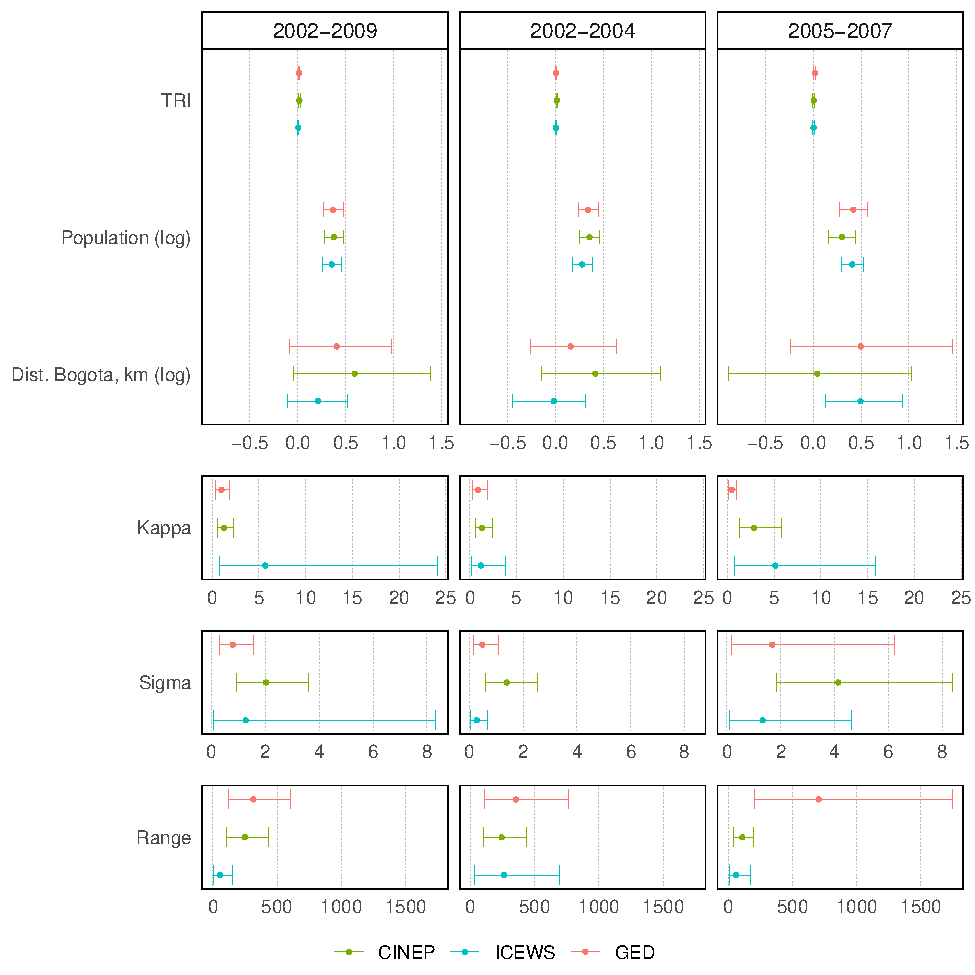
\includegraphics[width=1\linewidth]{INLA_Model_Tables_files/figure-latex/unnamed-chunk-6-1} \end{center}

\pagebreak

\hypertarget{coefficient-and-gmrf-parameter-plots-for-spde-models-of-undereporting-of-farc-hrvs}{%
\subsubsection{Coefficient and GMRF parameter plots for SPDE models of Undereporting of FARC HRVs}\label{coefficient-and-gmrf-parameter-plots-for-spde-models-of-undereporting-of-farc-hrvs}}

\hypertarget{icews-or-ged-in-comparison-with-cinep-in-indicated-periods}{%
\paragraph{ICEWS or GED in comparison with CINEP in Indicated Periods}\label{icews-or-ged-in-comparison-with-cinep-in-indicated-periods}}

\begin{center}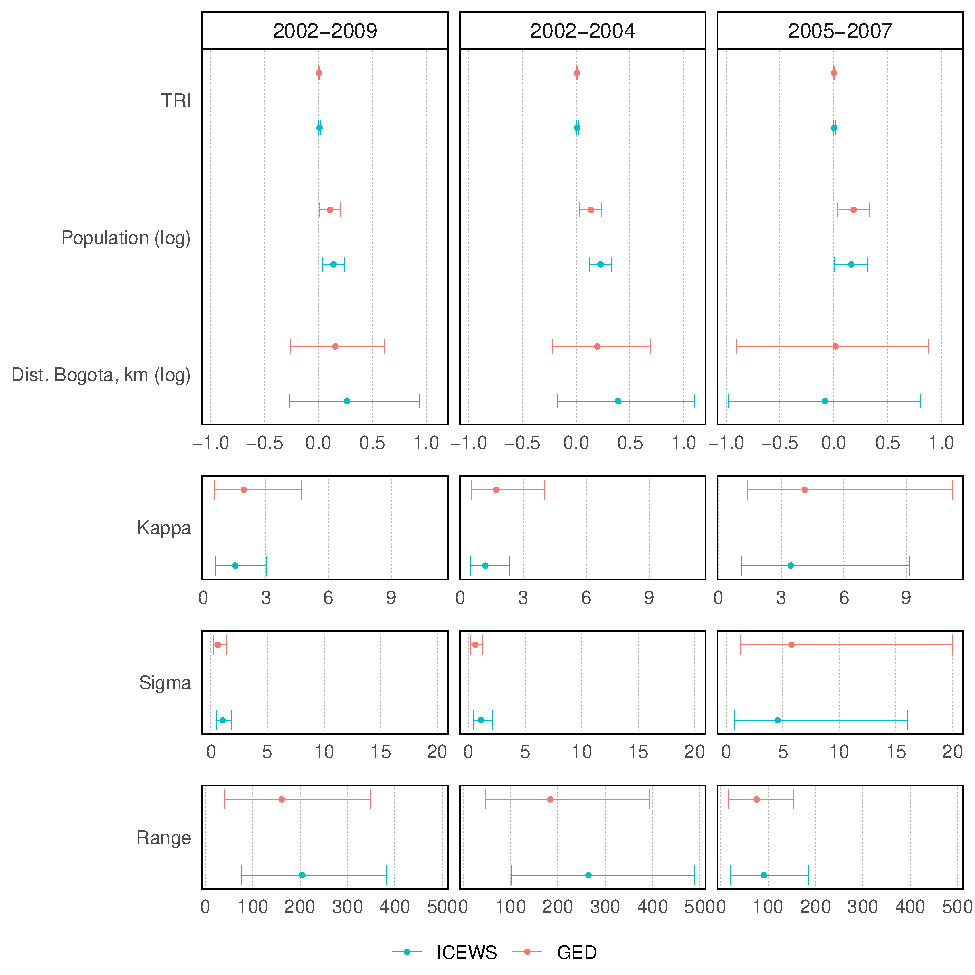
\includegraphics[width=1\linewidth]{INLA_Model_Tables_files/figure-latex/unnamed-chunk-7-1} \end{center}

\pagebreak

\hypertarget{colombia-map}{%
\section{Colombia Map}\label{colombia-map}}

\begin{center}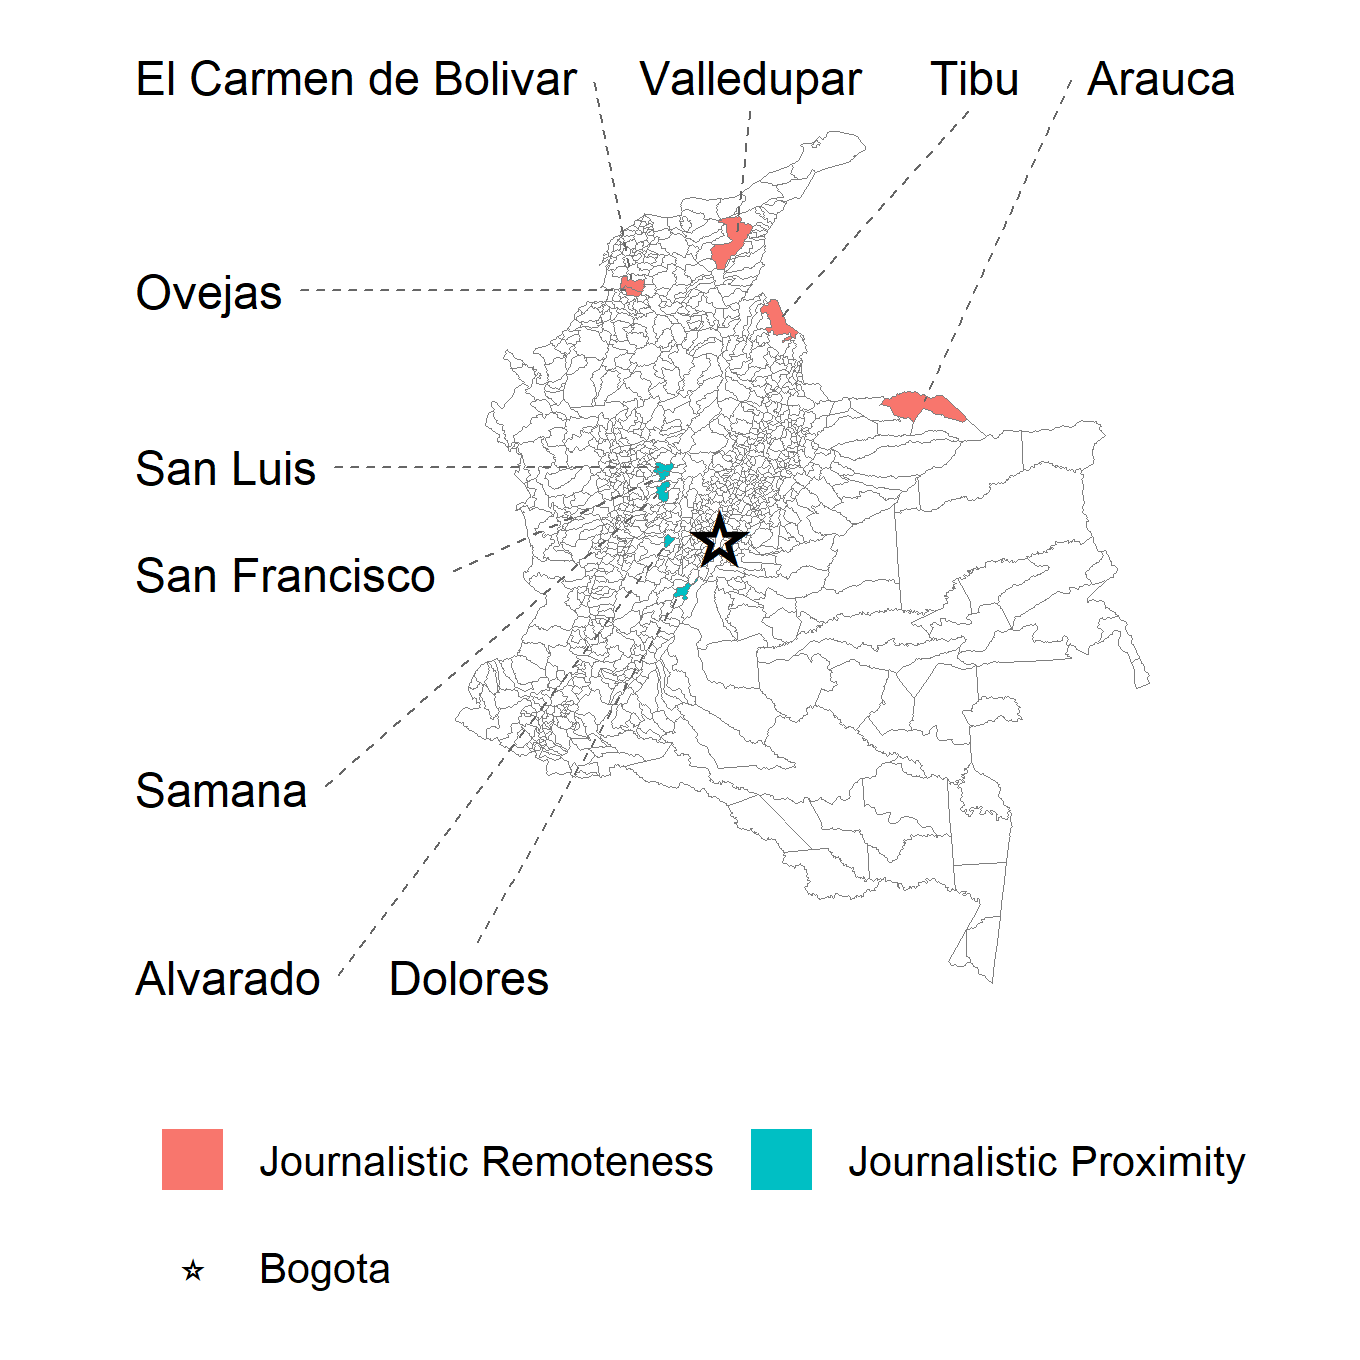
\includegraphics[width=1\linewidth]{Map} \end{center}

\end{document}
